% !TEX root = thesis.tex
\graphicspath{ {./figures/} }

%%%%%%%%%%%%%%%%
\chapter{Design}
\label{sec:design}
%%%%%%%%%%%%%%%%

This section describes our implementation of liquid democracy with fractional delegation. We start by defining delegation graphs, and introduce some constraints, after which we discuss what it entails resolve delegations.

\section{Implementing Liquid Democracy with Fractional Delegation}

\subsection{Delegation Graphs}

In our implementation, voters are strictly given the choice to either delegate their vote (fractional) in its entirety, or vote directly. The electorate is thus divided into \textbf{sinks}, who actually vote, and \textbf{delegators}. 

\section{Resolving Delegation}


\TODO{The stuff below was pasted from the old background, it needs to be severely adapted...}

\section{Liquid Democracy with Fractional Delegation}

In a liquid democracy, voters are given the choice between voting themselves, and delegating their vote to another voter, who will vote on their behalf. This distinguishes the electorate into "sinks", who actually vote, and "delegators".  In this paper, we will look at a fractional implementation of liquid democracy, which allows delegators to split their one vote into fractions and delegate those to different people.

 \TODO{Can be made longer}

 \section{Delegation Graphs}
 
In order to facilitate communication, a fractional amount of votes is also referred to as \textbf{power}. Each node initially has one vote, or an \textbf{initial power} $p^{(0)}_v = 1$. Each \textbf{delegation} between two nodes has a \textbf{weight} $w \in \mathbb{R}^+$.  \textbf{Resolving delegations} means to determine how much power each sink holds according to the delegations. After resolving delegations, a node $v \in V'$s \textbf{final power}, is $p_v \in \mathbb{R}_{\ge0}$. A more rigid definition of a nodes final power will be introduced in \cref{sec:design}.

This paper uses the a fractional implementation of liquid democracy, where each voter is either a \textbf{sink} or a \textbf{delegator}. This means that either the voter votes themselves, or chooses to delegate their vote fractionally. \textbf{Fractional delegation} allows the delegator to delegate (different) fractions of their initial vote to different voters. It is important to note, that since a node can only be either a delegator or a sink, it can't vote and delegate at the same time, so a sink can't delegate any power at all, and a delegator can't vote themselves. 
 
We define a \textbf{delegation graph} as a finite, directed, weighted graph $G = (V, E)$, with sinks $S$ and delegators $D$ as follows:

\begin{enumerate}
\item $V = S \dot\bigcup D$, meaning that $V$ is the union of the two disjunct sets of sinks and delegators.
\item Each $e \in E$ is a triple $(u, v, w)$, denoting a delegation from node $u$ to node $v$ of weight $w$.
\item Each sink $s \in S$ has no outgoing edges.
\item Each delegator $d \in D$ has $n \in \mathbb{N}^+$ outgoing edges, each with a positive weight \footnotemark, such that the sum of all outgoing edge weights equals 1.
\item Each voter $v \in V$ has corresponding power value, which is initially 1.
\end{enumerate}

\subsection{Closed Delegation Cycles}

\footnotetext{Edge weights should not be 0, since the edge should be entirely omitted in this case.}

We define a \textbf{closed delegation cycle} $C \subseteq V$ in a delegation graph $G = (S \dot\bigcup D, E)$ as a cycle in $G$ such that for every node $v \in C$, there exists no path from $v$ to any sink node in $S$. That is,
\[
\forall v \in C,\ \nexists\ \text{path from } v \text{ to any } s \in S.
\]

\begin{figure}[h]
    \centering
    \begin{subfigure}[t]{0.32\textwidth}
        \centering
        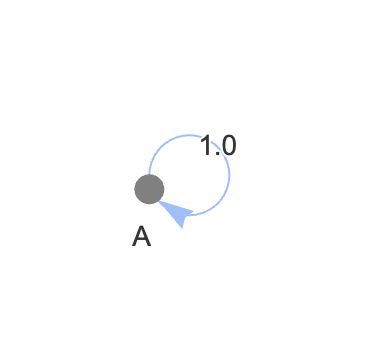
\includegraphics[width=\textwidth]{invalid_graph_1}
    \end{subfigure}
    \hfill
    \begin{subfigure}[t]{0.32\textwidth}
        \centering
        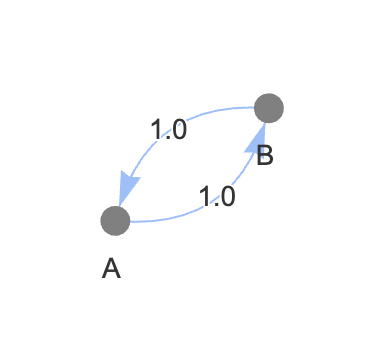
\includegraphics[width=\textwidth]{invalid_graph_2}
    \end{subfigure}
    \hfill
    \begin{subfigure}[t]{0.32\textwidth}
        \centering
        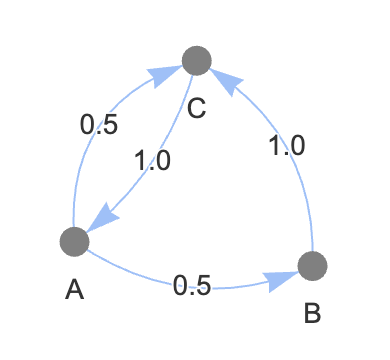
\includegraphics[width=\textwidth]{invalid_graph_3}
    \end{subfigure}
    \caption{Closed delegation cycles}
    \label{fig:closed-delegation-cycles}
\end{figure}

\Cref{fig:closed-delegation-cycles} shows exemplary cycles which are not allowed. Such cycles would lead to contradictory situations, as power delegated within them would never reach a sink. Some existing works discuss possible ways to handle this "lost" power \cite{behrensCircularDelegationsMyth2015, brillInteractiveDemocracy2018}, but it is out of the scope of this paper to provide comment on these. We prove below, that if there are no closed delegation cycles in a delegation graph, all delegators' power reaches a sink.

\begin{theorem}
Let $G = (S \dot\bigcup D, E)$ be a delegation graph. If $G$ contains no closed delegation cycles, then for every delegator $d \in D$, there exists a path from $d$ to a sink node $s \in S$.
\end{theorem}
\begin{proof}
Suppose, for contradiction, that $G$ contains no closed delegation cycle, but $\exists d \in D$ such that no path from $d$ leads to any sink $s \in S$. Since G is a finite graph, any walk from $d$ must eventually repeat nodes, implying a cycle. If at least one node in this cycle can reach a sink, there would be a path for all others in the cycle to reach a sink via this node as well, thus all nodes in the cycle can not reach a sink either. Thus, G does contain a closed delegation cycle. $\lightning$
\end{proof}

 A \textbf{well-formed delegation graph} G is defined as a delegation graph, which contains no closed delegation cycles.

 Note, that while a self loop of weight one is not allowed in a well-formed delegation graph, a self loop of weight $w \le 1$ is allowed as long as the rest of the node's power eventually flows to a sink. Since a delegator can't vote, any power a delegator delegates to themselves will "flow" back into the node, and then be redistributed to the nodes delegates. How the delegations are actually resolved will be covered in greater detail in \cref{sec:design}. 
 
 \section{Conservation of Power}
 
 A vital property we set for the delegation graph is the conservation of power. While some authors have experimented with implementations of liquid democracy where this is not the case \cite{bersetcheGeneralizingLiquidDemocracy2022, boldiViscousDemocracySocial2011}, we believe that for a system to be truly democratic, we must assert delegating is not penalised, so a vote cast by a sink should not be different in value to a vote cast by a sink through delegation from a delegator. This property is called "Equality of Direct and Delegating Voters" by Behrens and Swierczek \cite{behrensPreferentialDelegationProblem2015}.  
 Thus, any implementation needs a mechanism to ensure that the sum of the final power of all sinks is equal to the sum of the initial power of all nodes.
 
 We posit, for the moment intentionally vaguely, that for a well-formed delegation graph $G=(S \dot\bigcup D, E)$, after resolving delegations, the following assertions must hold.

\begin{enumerate}
\item $\forall s \in V$: $p_s = p$, where $p$ is the power delegated to $s$ directly or indirectly via its delegators.
\item $\forall d \in V$: $p_d = 0$ 
\item $\sum_{d \in D} p_d = |V|$
\end{enumerate}

\TODO{maybe prove these seven, or a subset of them: \url{https://liquid-democracy-journal.org/issue/3/The_Liquid_Democracy_Journal-Issue003-01-Preferential_Delegation_and_the_Problem_of_Negative_Voting_Weight.html}}

